\PassOptionsToPackage{svgnames}{xcolor}
\documentclass[a4paper,14pt]{article}

\input preamble.tex
\usepackage{systeme}
\usepackage{sectsty}
\usepackage{lipsum}
\usepackage{indentfirst}
\allsectionsfont{\centering\normalsize} % Заголовки с абзацного отступа: \indent %% по центру \centering
\subsectionfont{\normalsize\centering} % Подразделы с абзацного отступа + обычный шрифт

\begin{document}
\thispagestyle{empty}
\begin{center}
	Министерство сельского хозяйства РФ \\Федеральное государственное бюджетное образовательное учреждение\\ высшего образования
	\vspace{0.5ex}
	
	<<Пермский государственный аграрно-технологический университет\\ имени академика Д.Н. Прянишникова>>
\end{center}
\vspace{10ex}
\begin{tabularx}{\textwidth}{XX}
	& Кафедра менеджмента \\
%	& территориальной экономики
\end{tabularx}
\begin{center}
	\vspace{13ex}
	Контрольная работа\\
	по дисциплине <<Математическое моделирование в менеджменте>> \\
%	\vspace{1ex}
%	на тему <<Экономическая эффективность инвестиционной\\ деятельности предприятия на примере ООО <<Агрофирма Острожка>>
	\vspace{1ex}
	
	Вариант 9
\end{center}
	\vspace{8ex}
	\begin{tabularx}{\textwidth}{XX}
	& Выполнил:\\
	& студент факультета заочного \\
	& обучения по направлению \\
	& <<Менеджмент>> \\
	& Кузнецов Андрей Валерьевич \\
	& Шифр Мн-13-204\\
	& Руководитель:\\
	& к.э.н., доцент\\
	& Сафонов Алексей Юрьевич\\
	\end{tabularx}
\begin{center}
	\vfill
	Пермь 2019
\end{center}

\newpage
%\thispagestyle{empty}
%\begingroup
%	\centering{
		\tableofcontents
				%}
%\endgroup
			
		%

\newpage
\section{Тема 1. Устойчивость оптимизационного решения}

После того как оптимальное решение задачи найдено, проводится его экономико-математический анализ. Одним из его наиболее важных элементов является изучение того, как влияют на решение изменения различных параметров модели.

Такое исследование называется анализом устойчивости решения. Оно позволяет выяснить, насколько решение модели чувствительно к изменению внешних условий, а также определить область изменения параметров, в которой оно остается прежним.

Проиллюстрируем роль анализа устойчивости на примере задачи фирмы. Ее решение является наилучшим планом выпуска в конкретной экономической ситуации, которая характеризуется определенными условиями производства и сбыта продукции.

Они находят свое отражение в математической модели в виде фиксированных значений ее параметров: удельной прибыли изделий, наличных объемов ресурсов и нормативов их затрат.

При принятии решения ЛПР необходимо учитывать по крайней мере два обстоятельства: во-первых, значения параметров модели обычно известны неточно; во-вторых, часть из них, например прибыльность изделий, может измениться уже в ближайшем будущем

Поэтому если окажется, что небольшие изменения параметров сильно влияют на характеристики оптимального плана, то его реализация без дополнительного изучения модели не представляется разумной.

Это изучение должно включать уточнение значений параметров и области их вероятных изменений и может привести к заключению о необходимости корректировки самой модели.

Если же выяснится, что возможные колебания параметров мало или вообще не влияют на найденное решение, то его выбор в качестве плана производства будет более обоснованным.

Таким образом, анализ устойчивости должен предшествовать использованию результатов расчетов по модели при принятии управленческих решений.

Отчет по устойчивости содержит основную информацию для анализа устойчивости решения. Он состоит из двух таблиц (рис. ).

% Please add the following required packages to your document preamble:
% \usepackage{graphicx}
\begin{table}[!h]
	\caption{Отчет по устойчивости}
	\small
	\resizebox{\textwidth}{!}{%
		\begin{tabular}{|l|l|l|l|l|l|l|}
			\hline
			\multicolumn{7}{|l|}{\textbf{Изменяемые ячейки}}                                                                                                   \\ \hline
			\textbf{Ячейка} & \textbf{Имя}        & \textbf{Результ.} & \textbf{Нормир.}   & \textbf{Целевой}      & \textbf{Допустимое} & \textbf{Допустимое} \\
			&                     & \textbf{значение} & \textbf{стоимость} & \textbf{Коэффициент}  & \textbf{Увеличение} & \textbf{Уменьшение} \\ \hline
			\$B\$10         & Выпуск Изделие 1    & 56                & 0                  & 25                    & 1,1538              & 2,142 857           \\ \hline
			\$C\$10         & Выпуск Изделие 2    & 18                & 0                  & 40                    & 3,75                & 0,9375              \\ \hline
			\$D\$10         & Выпуск Изделие 3    & 0                 & -1,5               & 30                    & 1,5                 & 1E+30               \\ \hline
			\multicolumn{7}{|l|}{\textbf{Ограничения}}                                                                                                         \\ \hline
			\textbf{Ячейка} & \textbf{Имя}        & \textbf{Результ.} & \textbf{Теневая}   & \textbf{Ограничение}  & \textbf{Допустимое} & \textbf{Допустимое} \\
			&                     & \textbf{значение} & \textbf{цена}      & \textbf{Правая часть} & \textbf{Увеличение} & \textbf{Уменьшение} \\ \hline
			\$E\$5          & Сырье Расход        & 388               & 0                  & 400                   & 1E+30               & 12                  \\ \hline
			\$E\$6          & Оборудование Расход & 350               & 4                  & 350                   & 70                  & 30                  \\ \hline
			\$E\$7          & Труд Расход         & 480               & 1,5                & 480                   & 10,909              & 80                  \\ \hline
		\end{tabular}%
	}
\end{table}

Первая таблица <<Изменяемые ячейки>> содержит сведения о чувствительности оптимального решения и оптимального значения целевой функции к малым изменениям ее коэффициентов. Ее столбцы содержат следующую информацию:

<<Резулът. значение>> --- оптимальные значения переменных (объемы выпуска).

<<Нормир. стоимость>> --- двойственные оценки переменных, которые показывают, насколько изменится оптимальное значение целевой функ­ции, если принудительно включить единицу изделия этого вида в оптимальный план.

Эта оценка отлична от нуля лишь для изделий, не вошедших в оптимальный план. Так, оценка изделия 3 равна -1,5. Это означает, что если установить фирме обязательное задание по выпуску единицы этого изделия, т. е. заменить условие $x_3 \geq 0$ на $x_3 \geq 1$, то оптимальное значение прибыли уменьшится на 1,5 и составит 2118,5.

<<Целевой Коэффициент>> --- коэффициенты целевой функции (удельная прибыль изделия).

<<Допустимое Увеличение (Уменьшение)>> --- насколько можно увеличить (уменьшить) соответствующий коэффициент целевой функции (удельную прибыль изделия), чтобы оптимальное решение не изменилось.

Таким образом, при изменении первого коэффициента целевой функции (удельной прибыли изделия 1) в интервале $I_1= (22,86; 26,15)$ решение останется прежним.

Поэтому этот интервал называют интервалом устойчивости решения. Если же значение удельной прибыли выйдет за его пределы, то это приведет к изменению оптимального плана.% (см. ниже табл. 2.2).

Интервалы устойчивости для остальных коэффициентов целевой функции таковы:

\[ I_2 = (39, 06 ; 43,75)\ \text{и} \  I_3 = ( -\infty ;31,5). \]

Во второй таблице <<Ограничения>> находится информация об оптимальных оценках ограничений. Ее столбцы содержат следующие сведения:

<<Результ. значение>> --- значение левой части ограничения (затраты ресурсов) в оптимальном плане.

<<Теневая Цена>> --- двойственные оценки ограничений (ресурсов), показывающие, насколько изменится оптимальное значение целевой функции, если увеличить на единицу правую часть ограничения (наличный объем ресурса).

Таким образом, ресурсы имеют следующие оценки: сырье -0, оборудование -4 и труд -1,5. Это означает, что дополнительная единица сырья не приведет к увеличению прибыли фирмы, дополнительная единица оборудования позволит фирме увеличить свою прибыль на 4 единицы, а труда --- на 1,5 единицы



<<Ограничение Правая часть>> --- значения правых частей ограничений (наличные объемы ресурсов).

<<Допустимое Увеличение (Уменьшение)>> --- насколько можно увеличить (уменьшить) правую часть соответствующего ограничения, чтобы не изменилась его двойственная оценка (теневая цена).

Информация, содержащаяся в последних трех столбцах, позволяет найти интервалы устойчивости оценок, в пределах которых их значения не изменяются. Левая граница интервала вычисляется по формуле

<<Ограничение Правая часть>> -- <<Допустимое Уменьшение>>, а правая граница --- по формуле:

<<Ограничение Правая часть>> + <<Допустимое Увеличение>>.

Таким образом, интервал устойчивости оценки сырья имеет вид $J_1 = (388; +\infty)$. В нем оценка равна 0, так как этот ресурс избыточен. Ин­тервал устойчивости оценки оборудования $J_2 = (320; 420)$.

В его пределах каждая дополнительная единица оборудования позволяет фирме увеличить прибыль на 4 единицы. Соответственно, интервал устойчиво­сти оценки труда $J_3 = (400; 490,9)$.

\newpage
\section{Тема 2. Трендовые модели на основе кривых роста}

Использование метода экстраполяции на основе кривых роста для прогнозирования базируется на двух предположениях:
\begin{itemize}
	\item временной ряд экономического показателя действительно имеет тренд, т.е. преобладающую тенденцию;
	\item общие условия, определявшие развитие показателя в прошлом, останутся без существенных изменений в течение периода упреждения.
\end{itemize}

В настоящее время насчитывается большое количество типов кривых роста для экономических процессов. Чтобы правильно подобрать наилучшую кривую роста для моделирования и прогнозирования экономического явления, необходимо знать особенности каждого вида кривых. Наиболее часто в экономике используются полиномиальные, экспоненциальные и S-образные кривые роста. Простейшие полиномиальные кривые роста имеют вид:

\[ \hat{y_t} = a_0 + a_1t \ \text{(полином первой степени)}\]
\[ \hat{y_t} = a_0 + a_1t +a_2t^2 \ \text{(полином второй степени)}\]
\[ \hat{y_t} = a_0 + a_1t +a_2t^2 + a_3t^3 \ \text{(полином третьей степени)}\]
и т.д.

Параметр $а_1$ называют линейным приростом, параметр $а_2$ --- ускорением роста, параметр $а_3$ --- изменением ускорения роста.

Для полинома первой степени характерен постоянный закон роста. Если рассчитать первые приросты по формуле $u_t = y_t - y_{t-1}, t = 2, 3, ..., n$, то они будут постоянной величиной и равны $a_1$.

Если первые приросты рассчитать для полинома второй степени, то они будут иметь линейную зависимость от времени и ряд из первых приростов $u_2, u_3, ...$ на графике будет представлен прямой линией. Вторые приросты $u_t^{(2)} = u_t - u_{t-1}$ для полинома второй степени будут постоянны.

Для полинома третьей степени первые приросты будут полиномами второй степени, вторые приросты будут линейной функцией времени, а третьи приросты, рассчитываемые по формуле $u_t{(3)} = u_t^{(2)} - u_{t-1}^{(2)}$, будут постоянной величиной.

На основе сказанного можно отметить следующие свойства полиномиальных кривых роста:
\begin{itemize}
	\item от полинома высокого порядка можно путем расчета последовательных разностей (приростов) перейти к полиному более низкого порядка;
	\item значения приростов для полиномов любого порядка не зависят от значений самой функции $\hat{y_t}$.
\end{itemize}

Таким образом, полиномиальные кривые роста можно использовать для аппроксимации (приближения) и прогнозирования экономических процессов, в которых последующее развитие не зависит от достигнутого уровня.

В отличие от использования полиномиальных кривых использование экспоненциальных кривых роста предполагает, что дальнейшее развитие зависит от достигнутого уровня, например, прирост зависит от значения функции. В экономике чаще всего применяются две разновидности экспоненциальных (показательных) кривых: простая экспонента и модифицированная экспонента.





























%\input{1-3glava}

\newpage
\section{Тема 3. Теория массового обслуживания и её применимость в исследовании менеджмента}

Теория массового обслуживания представляет собой область прикладной математики, использующую методы теории случайных процессов и теории вероятностей для исследования различной природы сложных систем. Теория массового обслуживания непосредственно не связана с оптимизацией. Назначение ее состоит в том, чтобы на основе результатов наблюдений за «входом» в систему предсказать ее возможности и организовать наилучшее обслуживание для конкретной ситуации и понять, как последнее отразится на стоимости системы в целом. 

Для систем, относящихся к системам массового обслуживания, существует определенный класс задач, решение которых позволяет ответить на актуальные для сегодняшнего времени вопросы. С какой интенсивностью должно проходить обслуживание или должен выполняться процесс при заданной интенсивности и других параметрах входящего потока требований, чтобы минимизировать очередь или задержку в подготовке документа или другого вида информации? Какова вероятность появления задержки или очереди и ее величина? Сколько времени требование находится в очереди и каким образом минимизировать его задержку? Какова вероятность потери требования (клиента)? Какова должна быть оптимальная загрузка обслуживающих каналов? При каких параметрах системы достигаются минимальные потери прибыли? К этому перечню можно добавить еще целый ряд задач.

Система массового обслуживания (СМО) включает следующие структурообразующие объекты: источник требований; входной поток требований (поступление заявок); очередь; обслуживающую систему как совокупность каналов обслуживания заявок; выходной поток (обслуженные заявки или удовлетворенные требования). Рассмотрим их модели.

Источник требований. По месту нахождения источника, формирующего требования, СМО делятся на разомкнутые, когда источник находится вне системы, и замкнутые, когда источник находится внутри системы.

Входной поток требований. Подавляющее большинство теоретических разработок по исследованию систем массового обслуживания выполнено для условия, когда входной поток требований является пуассоновским (простейшим). Этот поток обладает рядом важных свойств. Он стационарен, ординарен и не имеет последствий.

Модель входного пуассоновского потока представляется функцией вида:
\[P_n(T) = \dfrac{(\lambda T)^ne^{\lambda T}}{n!},\]
где $ P_n(T)  $ --- вероятность поступления требований в течение заданного интервала времени $T$; \\
$\lambda$ --- интенсивность поступления требований в систему, т.е. математическое ожидание числа требований, поступивших за единицу времени:
\[\lambda =  \dfrac{1}{M(t)},\]
где $M(t)$ --- математическое ожидание случайной величины $t_i$, равной интервалу времени между $i$ и $i + 1$ поступлениями требований в систему; \\
$\lambda T$ --- математическое ожидание количества требований в период $T$; \\
$n$ --- количество поступлений требований в систему.

Следующее важное для исследования свойство, которым обладает пуассоновский поток, заключается в том, что процедура разделения и объединения дает снова пуассоновские потоки. Тогда, если входной поток формируется из $N$ независимых источников, каждый из которых порождает пуассоновский поток интенсивностью $\lambda_i (i=1,2,..., N),$ то его интенсивность будет определяться по формуле:
\[\lambda = \lambda_1 + \lambda_2 + ... + \lambda_N.\]

В случае разделения пуассоновского потока на $ N $ независимых потоков получим, что интенсивность потока $\lambda_i$ будет равна $r_i \lambda$, где $r_i$ --- доля $i$-го потока во входном потоке требований.

Очередь. Очереди, определяемые как множество требований, ожидающих обслуживания, представляются несколькими моделями: очередь с отказами, с ограниченным временем ожидания (заявка ждет определенное время), ограниченной длиной и, наконец, неограничен-ным временем ожидания. Порядок поступления заявок на обслуживание называется дисциплиной очереди. Требования могут приниматься по мере поступления, случайным порядком, с приоритетом, по принципу «последняя --- первой», по определенным каналам.

Процесс обслуживания. Основным параметром процесса обслуживания считается время обслуживания требования каналом $j$ --- $t_j(j =1,2,...,m)$. Величина $\uptau_j$ в каждом конкретном случае определяется рядом факторов: интенсивностью поступления заявок, квалификацией исполнителя, технологией работ, окружающей средой и т.д. Законы распределения случайной величины $\uptau_j$ могут быть самыми различными, но наибольшее распространение в практических приложениях получил экспоненциальный закон распределения. Функция распределения случайной величины $\uptau_j$ имеет вид:
\[F(t)=1-e^m,\]
где $m$ --- положительный параметр, определяющий интенсивность обслуживания требований;
\[m=\dfrac{1}{E(t)},\]
где $E(t)$ --- математическое ожидание случайной величины обслуживания требования $\uptau_j$.

Важнейшее свойство экспоненциального распределения заключается в следующем. При наличии нескольких однотипных каналов обслуживания и равной вероятности их выбора при поступлении заявки распределение времени обслуживания всеми $m$ каналами будет показательной функцией вида:
\[F(\uptau) = 1-e^{(\mu_1 +\mu_2 + ... + \mu_m)_{\uptau}}.\]

Если СМО состоит из неоднородных каналов, то $\mu = \sum\limits_{j=1}^m\mu_j$, если же все каналы однородные, то $\mu = m \mu_j$.

Выходной поток обслуженных требований. Выходной поток — это поток результатов деятельности, представленных выполненными требованиями в виде той или иной продукции или услуги. К основным параметрам выходного потока относятся интенсивность выхода из системы обслуженных требований и характер распределения времени между моментами выпуска продукции. В общем случае эти параметры определяются моделью входного потока, дисциплиной очереди и моделью обслуживания. Для СМО с параллельными каналами и однофазным обслуживанием существует теорема о том, что при пуассоновском входном потоке с параметром X и одинаковым для каждого канала распределением времени обслуживания с параметром ц в стационарном состоянии выходной поток имеет пуассоновское распределение с параметром g.

В многофазных системах выходной поток одного канала служит входным потоком для другого канала.

Особенность моделей СМО связана с достаточно строгим математическим описанием функционирования систем, что достигается благодаря их унификации по ряду признаков. Так, в зависимости от модели ожидания требованием начала обслуживания различают следующие СМО:
\begin{itemize}
	\item системы с потерями или отказами;
	\item системы с ожиданием;
	\item системы с ограниченным временем ожидания (ВО);
\item системы с ограниченной длиной очереди (ДО).
\end{itemize}

По числу каналов обслуживания системы делятся на одноканальные (т = 1) и многоканальные (т > 1). Одной из форм классификации СМО служит кодовая классификация Д. Кендалла. В соответствии с этой классификацией характеристику СМО записывают в виде трех, четырех или пяти символов. Например, а/Ь/с, где а — тип распределения входного потока требований, Ъ — тип распределения времени обслуживания, с — число каналов обслуживания. Для пуассоновского и экспоненциального распределений принимают символ М, для любого произвольного распределения — символ в. Например, запись М/М/2 означает, что входной поток требований пуассоновский, время обслуживания распределено по экспоненциальному закону, в системе имеются два канала. Четвертый символ (Модели СМО могут быть детерминированными или вероятност-ными. В первом случае параметры и переменные модели — это посто-янные величины, во втором — случайные.

Исследование СМО заключается в нахождении показателей, харак-теризующих качество и условия работы обслуживающей системы и показателей, отражающих экономические последствия принятых ре-шений согласно первым показателям. К показателям первой группы относятся следующие.

Рассмотрим приемы вычисления показателей первой группы на примере наиболее распространенной модели СМО (М/М/т > 2) с ожиданием, содержащей т параллельных обслуживающих каналов. Здесь поступающие требования не теряются и оставляют систему лишь после обслуживания. Каналы выполняют однородные операции, и время обслуживания каждым каналом * распределено по экспоненциальному закону с параметром т (10.5), а входящий поток — пуассоновский с параметром X (10.1); дисциплина очереди не регламентирована, и отсутствует ограничение на число поступающих требований. Модель СМО представляется в виде системы уравнений для стационарного состояния.

Пример. Требуется провести оценку эффективности централизации нескольких отделов или служб с однородными функциями. В качестве объекта рассматриваются две службы такси, которые приобрела компания «Автосервис». Заявки клиентов между службами распределяются поровну. Спрос на такси к диспетчеру поступает с частотой 10 вызовов в час. Среднее время обслуживания одного клиента составляет 11,5 мин. Вызовы такси распределены во времени по пуассоновскому закону, а продолжительность обслуживания одного клиента — по экспоненциальному закону. Каждая служба такси оснащена двумя автомобилями.

Возникает вопрос об экономической целесообразности централи-зации управления таксопарком. Для этого необходимо сравнить два варианта:
\begin{enumerate}
	\item вариант с независимым обслуживанием системами типа (М/М/2) при51= 10 вызовов/ч,т = 11,5мин. ит = 2;
	\item вариант с одной очередью типа (М/М/4) при X = 10 • 2 = 20 вызовов /ч, т — 11,5 мин. и /и = 4.
\end{enumerate}

Приведенные оценки показывают, что централизация служб позволяет сократить среднее время ожидания клиентом вызванного по телефону такси примерно вдвое. Это не гарантия, что клиент откажется от заказа, но существенное сокращение времени ожидания. В дальнейшем, кроме создания единой службы такси, необходимо рассматривать вопросы увеличения парка такси. При решении задач с размерностью т > 5 методами теории массового обслуживания потребуется автоматизированное вычисление.

Подводя итоги, отметим, что теория массового обслуживания предоставляет исследователю множество разнообразных моделей и методов решения задач по повышению эффективности обслуживания по-
требителей, клиентов.

\newpage
\section{Тема 4. Игры в чистых стратегиях}

Антагонистические игры, в которых каждый игрок имеет конечное множество стратегий, называются матричными играми.

Итак, матричная игра --- это конечная игра двух лиц с нулевой суммой (т. е. сумма выигрышей игроков в каждой ситуации равна нулю). Такая игра полностью определяется матрицей
\[ H = \begin{pmatrix}
h_{11} & h_{12} & \dots & h_{1n} \\ 
h_{21} & h_{22} & \dots & h_{2n} \\ 
\dots & \dots & \dots & \dots \\ 
h_{m1} & h_{m2} & \dots & h_{mn}
\end{pmatrix}  \],
в которой строки соответствуют чистым стратегиям игрока 1, столбцы --- чистым стратегиям игрока 2, на их пересечении стоит выигрыш игрока 1 в соответствующей ситуации, т. е. ситуации $s = (i, j)$ соответствует выигрыш $H_1(s) \equiv H (i, j) =  h_{ij}$. Тогда выигрыш игрока 2 равен $H_2(s) = - H_1(s)$ для всех $s \in S$.

Здесь игрок 1 имеет $m$ стратегий, игрок 2 имеет $n$ стратегий. Такая игра называется $m\times n$‑игрой. Матрица $H$ называется матрицей игры или матрицей выигрышей (платежной матрицей).

Цель игрока 1 --- максимизировать cвой возможный выигрыш, при этом увеличение его выигрыша ведет к уменьшению выигрыша игрока 2 (так как игра антагонистическая). Аналогичное можно отметить и для игрока 2: увеличение его выигрыша ведет к уменьшению выигрыша игрока 1. Поэтому при выборе стратегии игрок 1 (разумный игрок, действующий рационально) будет руководствоваться следующими соображениями. При стратегии $i$ игрока 1 игрок 2 выберет стратегию $j_*$, максимизирующую его (игрока 2) выигрыш (тем самым минимизирующую выигрыш игрока 1):
\[ h_{ij*} = \min_j h_{ij}\].

Тогда оптимальная стратегия игрока 1, которая обеспечит ему наибольший из возможных выигрышей $h_{ij*}, i = 1, 2, ..., m$, (т. е. при любой стратегии игрока 2), будет состоять в выборе стратегии $i_*$, для которой выполняется:
\[ h_{i*j*} = \max_i h_{ij*} = \max_i \min_j h_{ij} \].

Аналогичными соображениями будет руководствоваться игрок 2 при выборе стратегии: обеспечить наибольший возможный выигрыш при любом выборе стратегии игрока 1, т. е. выбрать стратегию, которая обеспечит ему $max$ из возможных выигрышей
\[ -h_{i*j},j = 1, 2,..., n, \ \text{здесь} \ h_{i*j} = \max_i h_{ij} \],
причем для второго игрока выигрыш равен $–h$, где $h$ --- выигрыш игрока 1.

Таким образом, оптимальная стратегия игрока 2 будет состоять в выборе стратегии $j*$, для которой выполняется:
\[ -h _{i*j*} = \max_j (-h_{i*j}) = \max_j (-\max_i h_{ij}) = - \min_j \max_i h_{ij} \],
отсюда получим:
\[h_{i*j*} = \min_j \max_i h_{ij}\].

\newpage
\section{Тема 5. Сетевое планирование проекта}

Сетевое планирование и управление (СПУ), система планирования и управления разработкой крупных народно-хозяйственных комплексов, научными исследованиями, конструкторской и технологической подготовкой производства новых видов изделий, строительством и реконструкцией, капитальным ремонтом основных фондов путём применения сетевых графиков. Система СПУ позволяет устанавливать взаимосвязь планируемых работ и получаемых результатов, более точно рассчитывать план, а также своевременно осуществлять его корректировку. СПУ --- основа использования ЭВМ в управлении и создании АСУ.

Сущность СПУ состоит в составлении логико-математической модели управляемого объекта в виде сетевого графика (рисунок \ref{fig:seti}) или модели, находящейся в памяти ЭВМ, в которой отражаются взаимосвязь и длительность определённого комплекса работ. Сетевой график после его оптимизации средствами прикладной математики и вычислительной техники используется для оперативного управления работами.
\begin{figure}[!h]
	\centering
	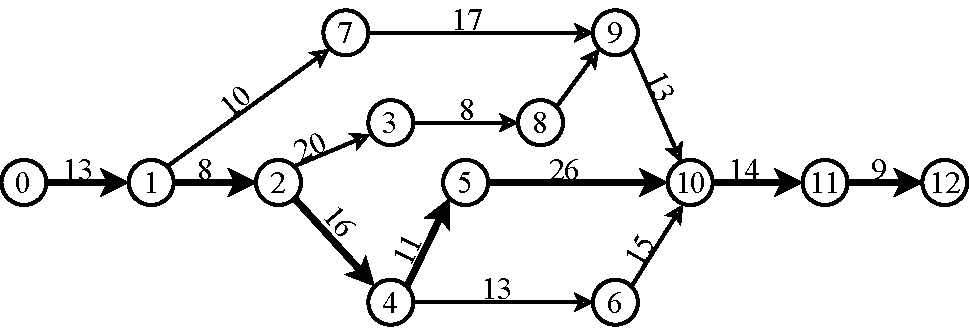
\includegraphics[width=0.7\linewidth]{seti}
	\caption{Сетевой график}
	\label{fig:seti}
\end{figure}

На график нанесены работы и события. Каждое событие характеризует завершение или начало работы, а работа означает действие, которое нужно совершить, чтобы перейти от предшествующего события к последующему. События на графике обозначаются кружками, а работы --- стрелками, показывающими связь между событиями (возможен и другой вариант: работы изображаются кружками, а связи между ними стрелками). Работа должна быть конкретной, четко описанной и иметь ответственного исполнителя; продолжительность её измеряется количеством дней, недель, декад и др., наносимых над стрелкой. Временные оценки даются ответственными исполнителями соответствующих работ. Все работы в графике ведут к конечному событию --- цели планирования.

При планировании длительности работ пользуются действующими нормативами и опытными данными, но во многих случаях (в частности, когда рассматриваются программы по освоению новых видов продукции или проблемные научные исследования) время работы не может быть выражено одной достоверной оценкой; ответственный исполнитель обычно даёт 3 оценки. Оптимистическая оценка времени (минимальная продолжительность работы $t_{min}$) --- минимальный срок, в течение которого будет выполнена работа в наиболее благоприятных условиях, если ничто не помешает её выполнению. Пессимистическая оценка времени (максимальная продолжительность работы $t_{max}$) характеризуется продолжительностью времени, необходимого для выполнения работы при наиболее неблагоприятных условиях, если в процессе её выполнения возникнут трудности. Наиболее вероятная продолжительность времени ($t_{\text{нв}}$) показывает время выполнения работы в нормальных условиях.

Ожидаемая продолжительность работы определяется на основании 3 или 2 оценок по одной из следующих формул:
\[t_{\text{ож}} =\dfrac{t_{min} + 4 \cdot t_{\text{нв}} + t_{max}}{6}\  \text{или} \  t_{\text{ож}} = \dfrac{3 \cdot t_{min}  +2 \cdot t_{max} }{5} \]
 

Важный элемент разработки сетевого графика --- определение продолжительности путей. На рисунке \ref{fig:seti} пути представлены линиями, образуемыми стрелками взаимосвязанных работ, концы которых указывают на начальные и конечные события. Различают полные и критические пути: полным называется путь, начало которого совпадает с исходным событием сети, а конец --- с её завершающим событием; критическим --- путь, имеющий наибольшую продолжительность и характеризующий время выполнения всего комплекса работ, проекта в целом, т. е. время достижения конечной цели (на рисунке обозначен жирными стрелками).

Критический путь расценивается как самый важный в системе СПУ, т. к. представляет собой основу для выбора оптимального плана и организации контроля за ходом работ. Отношение продолжительности любого пути к продолжительности критического пути характеризует степень его напряжённости. Если критический путь является наиболее продолжительным по времени от начального до конечного события, то все др. события и работы должны лежать на путях более коротких.

Совершенные формы СПУ содержат информацию относительно движения материальных затрат и наращивания издержек по объекту. СПУ проводится примерно в следующей очерёдности: расчленение комплекса работ на отдельные последовательные этапы, каждый из которых закрепляется за ответственным исполнителем; выявление и описание всех событий и работ, необходимых для достижения неконечной цели; построение сетевого графика; определение времени выполнения каждой работы в сети на основе системы оценок; расчёт критического пути и резервов времени; анализ сети и оптимизация графика, разработка мероприятий по сокращению времени критического пути; управление ходом работ с помощью сетевого графика.

Каждый исполнитель определяет состав и последовательность закрепленного за ним этапа работ. Затем ответственное за проект лицо составляет первичные сетевые графики, которые после их корректировки «сшиваются» в сводный сетевой график. Этот график завершается событием, соответствующим заданной конечной цели. При этом особое внимание уделяется устранению неувязок на стыках между первичными сетевыми графиками, т. е. этапами комплекса работ.

По мере движения ко всё более высокому уровню выполнения работ планы-графики укрупняются. Если они предназначены для руководителей предприятий, то в них включаются только сроки свершения граничных событий, являющихся выходными для одних предприятий и входными для других, с указанием времени начала и окончания работ критической зоны. Планы-графики руководителей промежуточных ступеней дополняются сведениями о сроках свершения граничных событий между отдельными ответственными исполнителями.

В процессе выполнения планов-графиков осуществляются непрерывный контроль, корректировка и регулирование сетевой модели. Для устранения расхождений между запланированным и фактическим ходом работ проводятся организационно-технические мероприятия.

Т. о., СПУ создаёт в конечном счёте условия для выполнения всего комплекса работ в их логической последовательности. С помощью сетевых графиков осуществляется системный подход к вопросам организации управления заданными процессами, поскольку коллективы различных подразделений участвуют в них как звенья единой сложной организационной системы, объединённые общностью задачи.
%\nocite{michurina,01,02,03,04,05,06,07,08,09,10}

\newpage
\renewcommand\refname{Список использованных источников}
\addcontentsline{toc}{section}{Список использованных источников}
\printbibliography
%\addcontentsline{toc}{section}{Приложения}
%\small{\listoftables}
%\addcontentsline{toc}{section}{Список таблиц}
%\newpage
%\thispagestyle{empty}
%\topskip0pt
%\vspace*{\fill}%
%\begin{center}
%	\textbf{ПРИЛОЖЕНИЯ}
%\end{center}
%\vspace*{\fill}
%
\end{document}
